\subsection{Entity-Relationship Schema}

 \begin{figure}[h!]
   \centering
   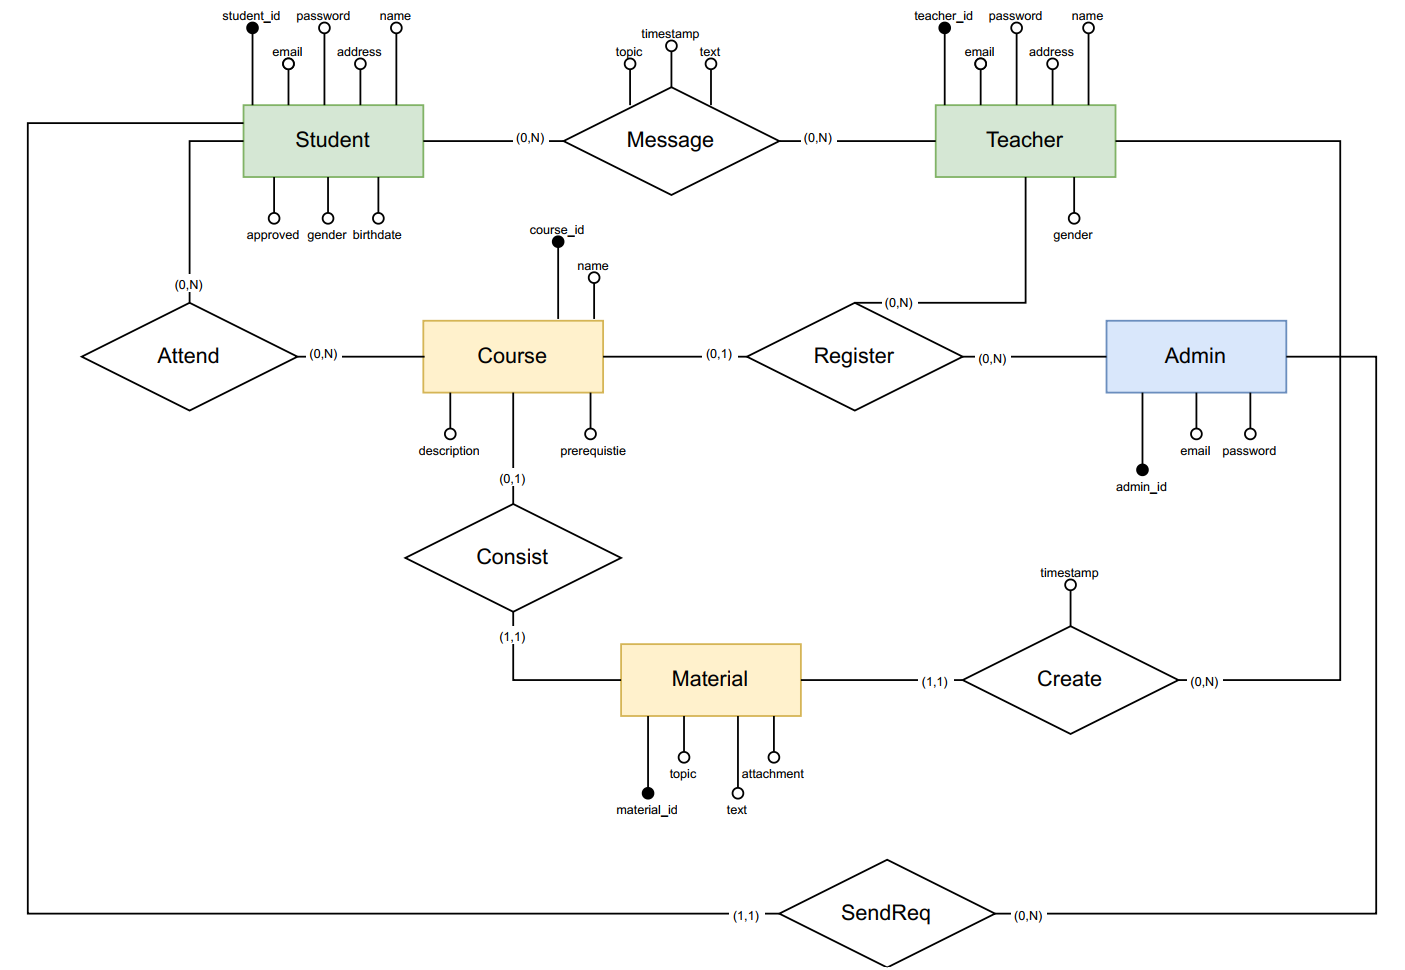
\includegraphics[width=17.7cm]{HW_1/images/FINAL-ER.png}
 \end{figure}
 
 %Describe here your ER schema 
The ER schema contains 5 main entities:
 \begin{itemize}
  \item Admin: This entity consists of the system admin and its primary key is an integer with auto-increment. Also, it has email(username) and password for logging into system as the admin user.
  \item Student: This entity is another type of the available users in the system. The primary key is an integer with auto-increment and in addition, there are some attributes used for logging into system (email, password) and personal information (name, gender, birth-date, address) for registering in the system. There is another Boolean attribute named as 'approved' which its value is set to true after the admin accepts the student's registration request.
  \item Course: This entity is the collection of courses available in the system for the students to enrol in. The primary key is an integer with auto-increment and the other attributes are used to save some information about each course.
  \item Teacher: Another type of users is the teacher entity which are registered (signed up) into system by the admin. Then one or more courses can be assigned to them.
  \item Material:Each course may have some materials (homeworks, announcements, etc). Therefore, they are all kept by having an integer auto-increment id for each material and their topic, text, and attachments if available are saved.
 \end{itemize}